\documentclass[conference]{IEEEtran}
\IEEEoverridecommandlockouts

\usepackage{cite}
\usepackage{amsmath,amssymb,amsfonts}
\usepackage{algorithmic}
\usepackage{graphicx}
\usepackage{textcomp}
\usepackage{xcolor}
\def\BibTeX{{\rm B\kern-.05em{\sc i\kern-.025em b}\kern-.08em
    T\kern-.1667em\lower.7ex\hbox{E}\kern-.125emX}}


\begin{document}

\title{Integrated Structures of Gravity Feedforward Terms in PD Control for a 6-DOF Mobile Manipulator}
\author{
	\IEEEauthorblockN{
		Lingyu Kong$^{\dagger}$,
		Haoran Xu$^{\dagger}$,
		Siyuan Zhou,
		Xingjian Li,
		Weizhong Li,
		Runmei Li$^{*}$
	}
	
	\IEEEauthorblockA{
		Beijing Jiaotong University, Beijing, China \\
	}
	
	\thanks{$^{\dagger}$ Lingyu Kong and Haoran Xu contributed equally to this work.}
	\thanks{$^{*}$ Corresponding author: Runmei Li (rmli@bjtu.edu.cn).}
	\thanks{This work was supported by Beijing Natural Science Foundation (L241055).}
}

\maketitle

\begin{abstract}
To improve tracking performance, gravity compensation is often introduced into the control of robotic arms based on phase shifter (PD) control. This paper studies three representative gravity compensation integrated structures within a unified PD control framework. Experiments were conducted on a six-DOF mobile robotic arm to evaluate their impact on transient response, steady-state accuracy, and robustness. The results show that different integrated structures exhibit different performance characteristics. For example, additive feedforward minimizes error when model accuracy is high; saturated injection is more stable when model error is large, but residual bias exists; integral type can eliminate bias but slows down transient response. This indicates that the integration method of gravity compensation plays a crucial role in practical robotic arm control.
\end{abstract}

\begin{IEEEkeywords}
	PD control, gravity compensation, feedforward control, integration structure, mobile manipulator, experimental comparison
\end{IEEEkeywords}



\section{Introduction}

Proportional--Derivative (PD) control is one of the most widely used control strategies for robotic manipulators due to its simple structure, intuitive parameter tuning, and satisfactory robustness in practical applications \cite{b1,b2}. However, in the presence of gravity effects, payload variations, and external disturbances, pure PD control generally exhibits non-negligible steady-state tracking errors. As a result, gravity compensation is commonly incorporated into PD-based controllers to improve tracking performance \cite{b3,b4}.

Existing studies on gravity compensation mainly focus on improving tracking accuracy or disturbance rejection performance, and a variety of implementation forms have been reported. These include additive feedforward compensation, saturation-based schemes with bounded inputs, and PD controllers augmented with nonlinear or integral actions \cite{b5,b6,b7,b8,b9}. While these approaches share similar control objectives, their implementations differ significantly in how gravity-related terms are incorporated into the control loop.

Despite extensive research on gravity compensation techniques, a systematic experimental comparison of different gravity compensation integration structures within a unified PD framework remains limited. In particular, how different integration forms influence transient behavior, steady-state accuracy, and sensitivity to model uncertainty has not been sufficiently clarified from an engineering perspective. From a structural perspective, gravity compensation is not merely an additional feedforward term, but implicitly reshapes the closed-loop error dynamics and the priority among performance objectives. Different integration structures inherently favor different trade-offs among steady-state accuracy, transient behavior, convergence speed, and tuning robustness, even under identical PD gains.


Motivated by this observation, this paper experimentally investigates three representative gravity compensation integration structures within a conventional PD control framework. Experiments are conducted on a six-degree-of-freedom mobile manipulator under identical control gains and reference trajectories. The results reveal consistent differences in performance characteristics and parameter sensitivity among the considered structures, highlighting the practical impact of gravity compensation integration choices.



The main contributions of this paper can be summarized as follows:
\begin{itemize}
	\item Three commonly used gravity compensation integration structures are implemented within a unified PD control framework and experimentally evaluated on a 6-DOF mobile manipulator.
	
	\item A structure-oriented gravity modeling formulation is adopted to support consistent implementation and comparison under identical experimental conditions.
	
	\item Experimental observations are interpreted using a Lyapunov-based analysis to provide insight into the performance differences among the considered compensation structures.
\end{itemize}


The remainder of this paper is organized as follows. 
Section~II describes the experimental platform and the gravity modeling framework used to support structural comparison. 
Section~III reports experimental results obtained under different gravity compensation integration structures within a unified PD framework. 
Section~IV provides a Lyapunov-based interpretation of the observed experimental phenomena. 
Section~V concludes the paper and discusses future research directions.



\section{Experimental Platform and Modeling Framework}
This section introduces the experimental platform and the gravity modeling framework adopted in this study.
Both the platform configuration and the modeling choices are intentionally designed to support a focused investigation of how gravity compensation terms are structurally integrated into a PD control framework, while minimizing confounding factors unrelated to gravity integration mechanisms.

\subsection{Experimental Platform Description}

\begin{figure}
	\centering
	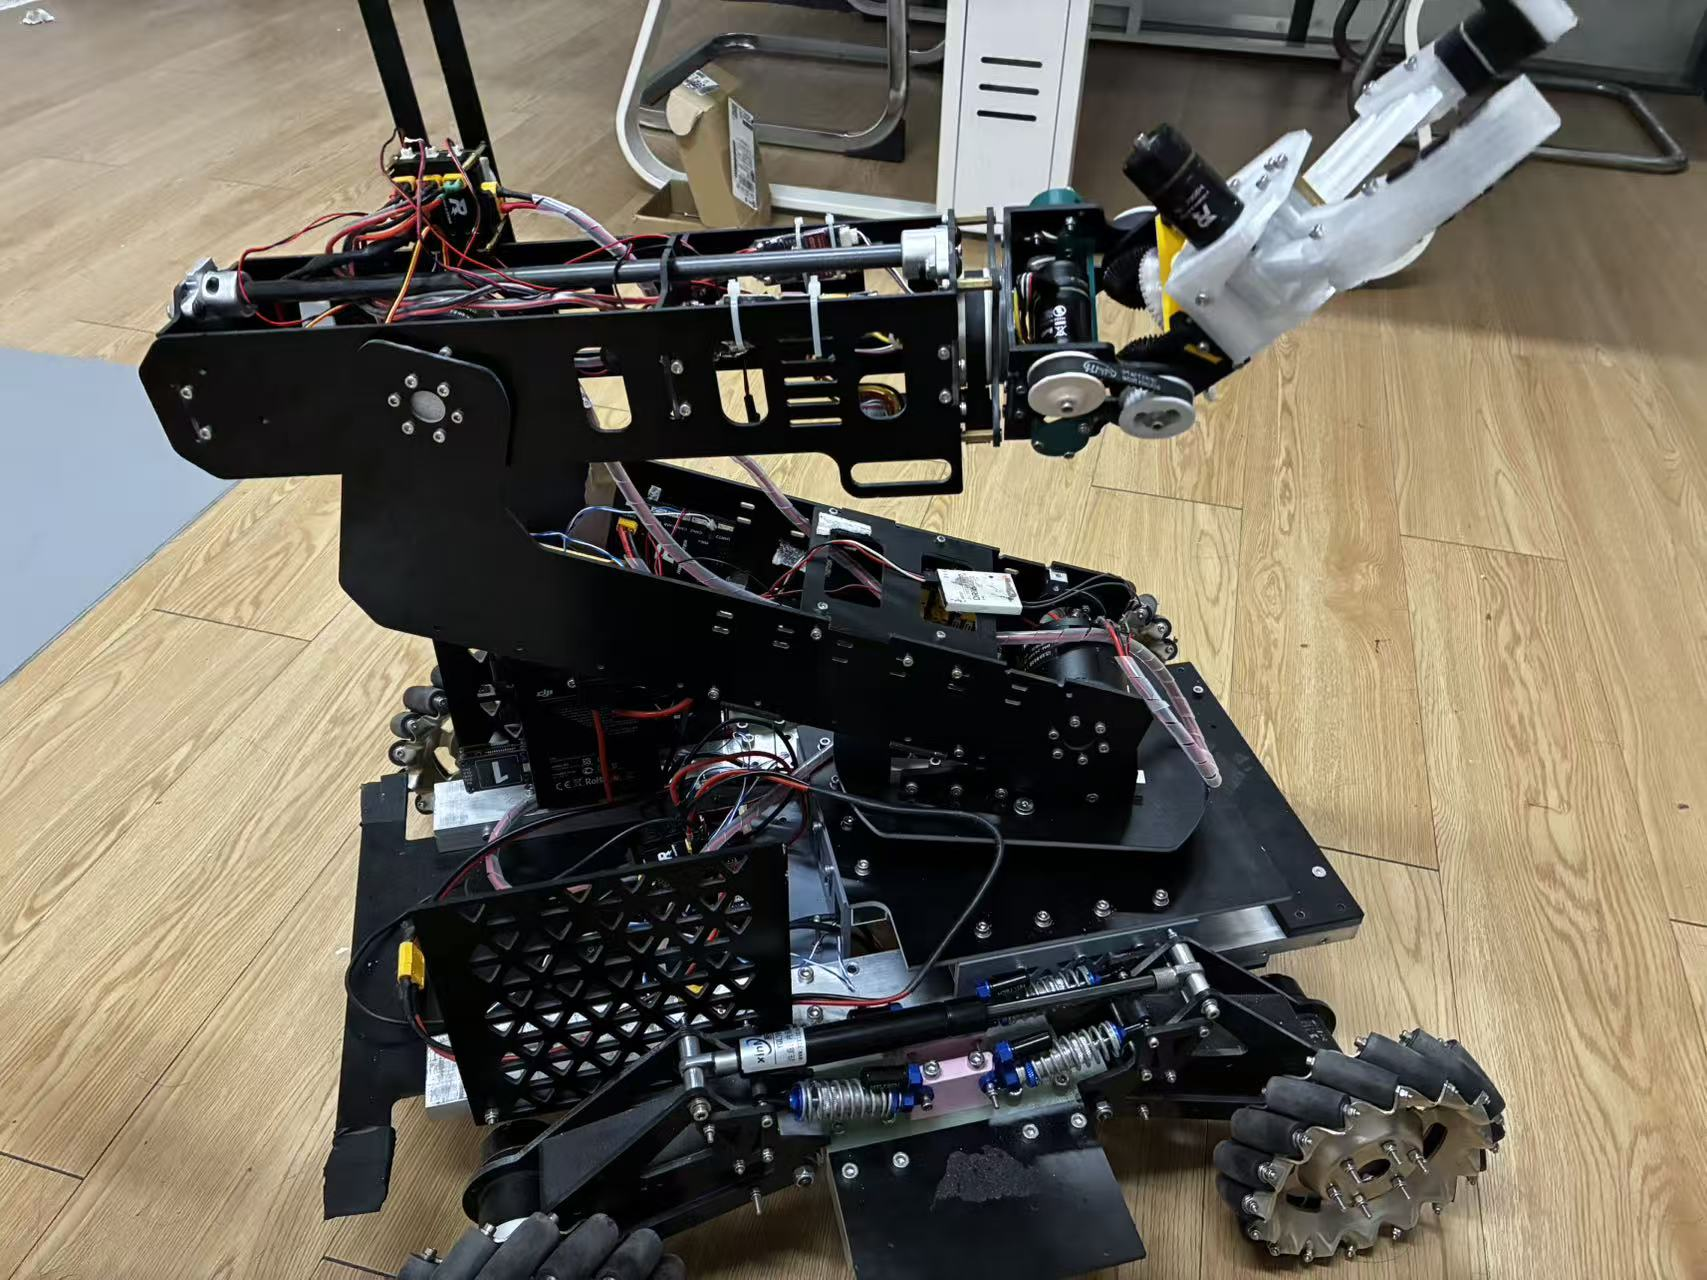
\includegraphics[width=0.7\linewidth]{pngs/Fig_1}
	\caption{Experimental platform of the 6-DOF mobile manipulator}
	\label{fig:fig1}
\end{figure}

The experiments are conducted on a six-degree-of-freedom (6-DOF) serial manipulator mounted on a mobile base equipped with four Mecanum wheels, as shown in Fig.~\ref{fig:fig1}. The mobile base enables planar omnidirectional motion, introducing bounded disturbances to the manipulator during operation.

Due to the mechanical structure and suspension of the base, variations in the vertical direction are negligible during planar motion. As a result, the orientation of the manipulator base frame remains approximately constant, and the direction of gravity can be assumed fixed throughout the experiments.

\subsection{Manipulator Dynamics under Moving-Base Disturbance}
The joint-space dynamics of the 6-DOF manipulator are described by the standard Euler--Lagrange formulation
\begin{equation}
	M(q)\ddot{q} + C(q,\dot{q})\dot{q} + G(q) = \tau + d(q,\dot{q},t),
\end{equation}
where $d(q,\dot{q},t)$ represents bounded disturbances induced by the motion of the mobile base.

In the considered experimental setup, the gravity direction relative to the manipulator base frame remains constant. Therefore, gravity-related effects are captured solely by the term $G(q)$, while base-induced effects are treated as disturbances.

\subsection{Gravity Modeling for Compensation}

The gravity-induced joint torque vector is derived from the gradient of the total gravitational potential energy,
\begin{equation}
	G(q) = \nabla_q U(q),
\end{equation}
ensuring physical consistency of the gravity model.

To facilitate implementation and structural comparison, the gravity term is formulated by exploiting the modular mechanical structure of the manipulator. Only joints that generate significant gravity-induced torques are considered in the compensation model.


\begin{figure}
	\centering
	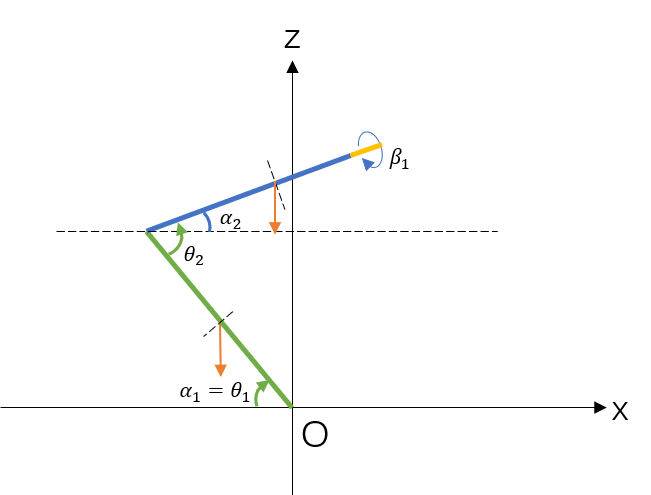
\includegraphics[width=0.8\linewidth]{pngs/Fig_2}
	\caption{Simplified planar structural decomposition of the manipulator for gravity modeling for joint1 and 2}
	\label{fig:fig2}
\end{figure}

\begin{figure}
	\centering
	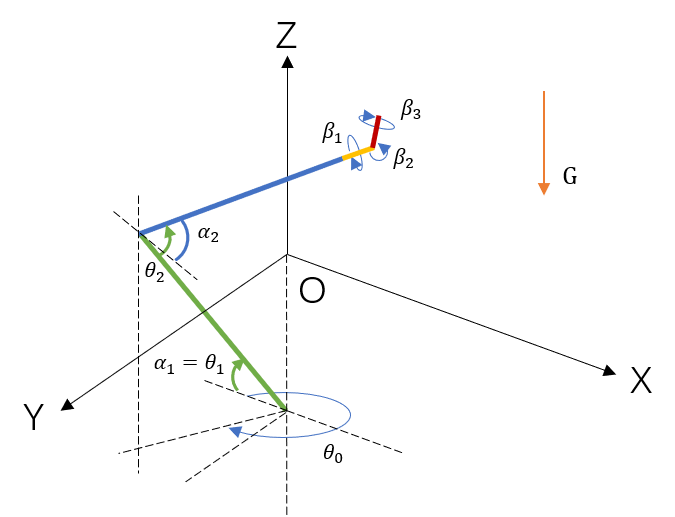
\includegraphics[width=0.8\linewidth]{pngs/Fig_3}
	\caption{Structural decomposition of the manipulator for gravity modeling in 3D space}
	\label{fig:fig3}
\end{figure}


Based on the potential energy formulation, the generalized gravity torque vector is given by
\begin{equation}
	G(q) = \frac{\partial U(q)}{\partial q}.
\end{equation}

The explicit expressions of the gravity torque components for each joint are derived accordingly and summarized as follows.

\paragraph{For the shoulder joint $\alpha_1$:}
\begin{equation}
	\begin{aligned}
		G_1 =\;&
		m_1 g \frac{l_1}{2} \cos \alpha_1
		+ m_2 g l_1 \cos \alpha_1
		+ m_2 g \frac{l_2}{2} \cos \alpha_{12} \\[2pt]
		&+ m_e g l_1 \cos \alpha_1
		+ m_e g l_2 \cos \alpha_{12} \\[2pt]
		&+ m_e g l_e \cos \alpha_{12} \cos \beta_2
		- m_e g l_e \sin \alpha_{12} \sin \beta_2 \cos \beta_1 .
	\end{aligned}
\end{equation}

\paragraph{For the elbow joint $\alpha_2$:}
\begin{equation}
	\begin{aligned}
		G_2 =\;&
		m_2 g \frac{l_2}{2} \cos \alpha_{12}
		+ m_e g l_2 \cos \alpha_{12} \\[2pt]
		&+ m_e g l_e \cos \alpha_{12} \cos \beta_2
		- m_e g l_e \sin \alpha_{12} \sin \beta_2 \cos \beta_1 .
	\end{aligned}
\end{equation}


\paragraph{For the wrist roll joint $\beta_1$:}
\begin{equation}
	G_3
	= - m_e g l_e
	\cos \alpha_{12} \sin \beta_2 \sin \beta_1 .
\end{equation}

\paragraph{For the wrist pitch joint $\beta_2$:}
\begin{equation}
	G_4
	= m_e g l_e \bigl(
	- \sin \alpha_{12} \sin \beta_2
	+ \cos \alpha_{12} \cos \beta_2 \cos \beta_1
	\bigr).
\end{equation}

The complete gravity compensation vector is thus given by
\begin{equation}
	G(q)=[G_1,G_2,G_3,G_4]^{\top}.
\end{equation}
which is consistent with the potential energy formulation and can be directly employed for gravity compensation within the PD control framework.


\subsection{Integrated Structures}
This section introduces three typical proportional-derivative (PD) based control structures, differing in how the gravity term is integrated into the control law. All controllers employ the same PD feedback loop structure.

\begin{figure}
	\centering
	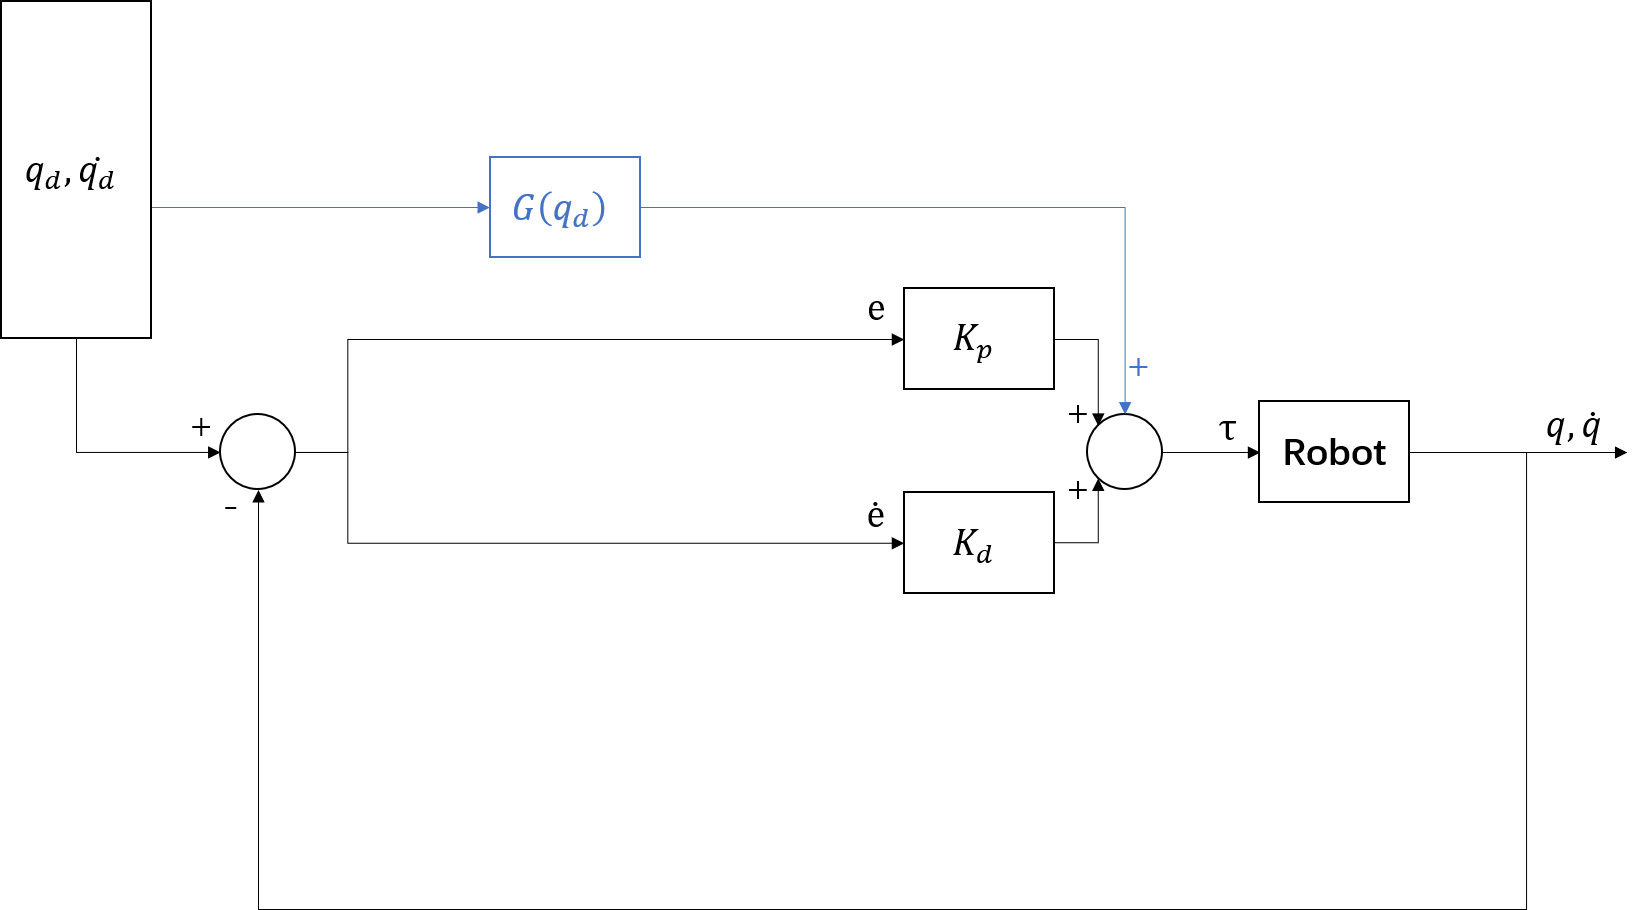
\includegraphics[width=0.7\linewidth]{pngs/Fig_4}
	\caption{PD control with additive gravity feedforward}
	\label{fig:fig4}
\end{figure}

\subsubsection{Additive Feedforward Method}

In the additive feedforward structure, gravity compensation is implemented as an explicit term added to the PD control law:
\begin{equation}
	\tau = -K_p e - K_d \dot{e} + \hat{G}(q),
\end{equation}
where $\hat{G}(q)$ denotes an estimate of the gravity torque vector.


\begin{figure}
	\centering
	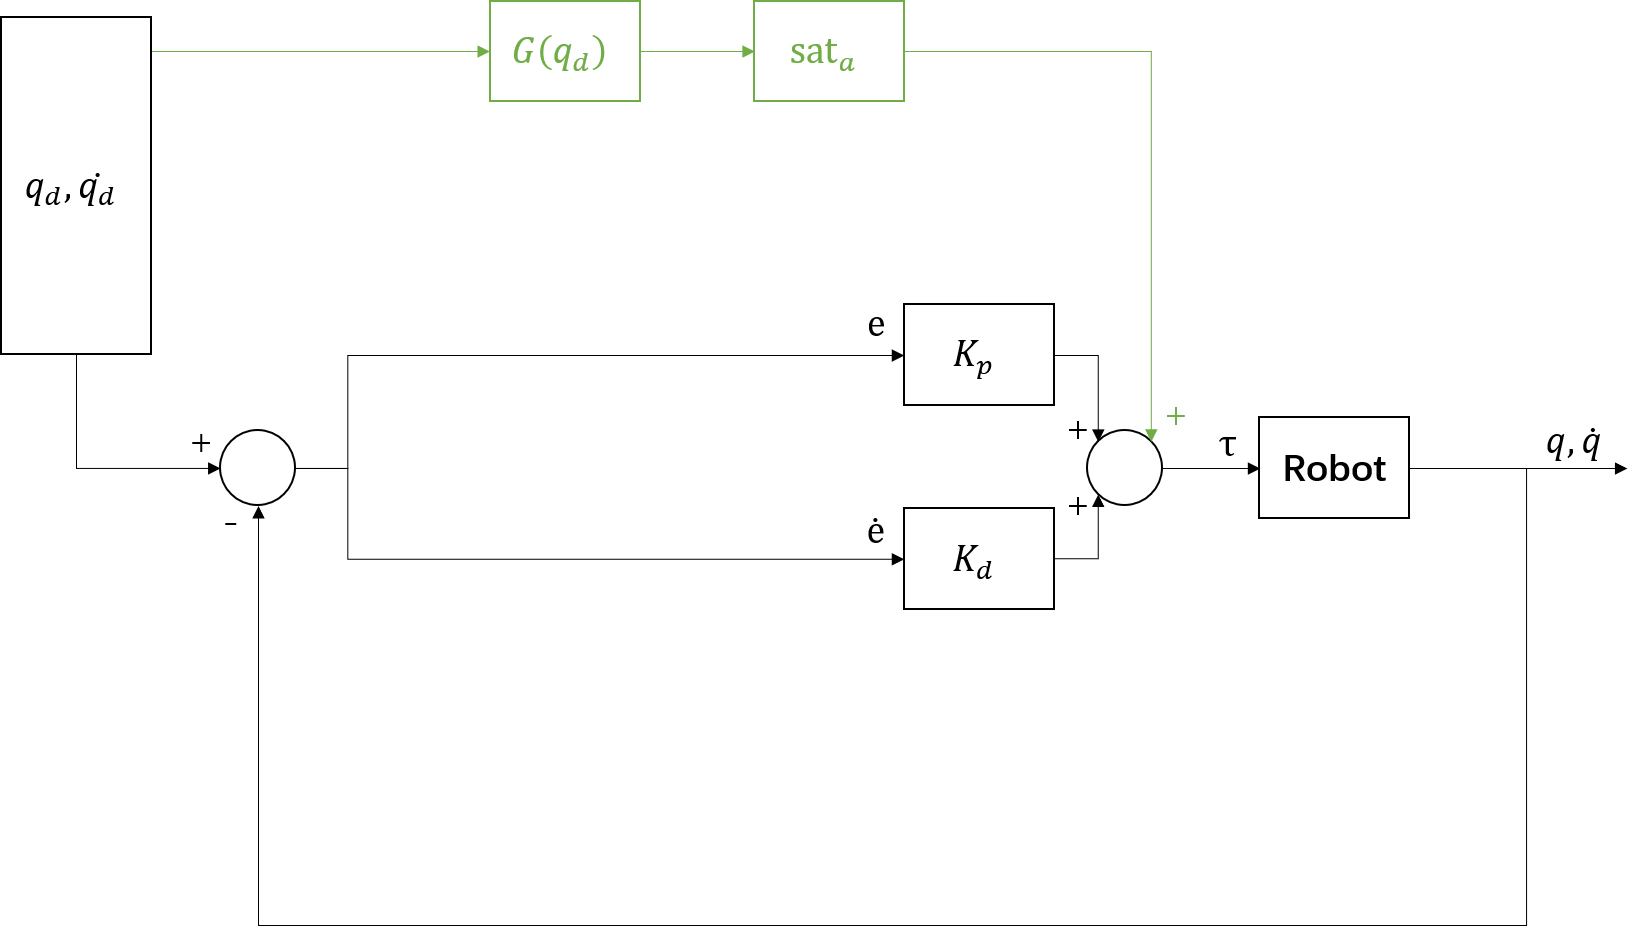
\includegraphics[width=0.7\linewidth]{pngs/Fig_5}
	\caption{PD control with saturation-based gravity compensation}
	\label{fig:fig5}
\end{figure}

\subsubsection{Saturation-Function Method}

In saturation-based structures, gravity compensation is constrained by a saturation function to limit its influence on the control input. Two commonly used formulations are considered:
\begin{equation}
	\tau = \mathrm{sat}\left( -K_p e - K_d \dot{e} + G(q) \right),
\end{equation}
\begin{equation}
	\tau = -K_p e - K_d \dot{e} + \mathrm{sat}\left( G(q) \right),
\end{equation}
where $\mathrm{sat}(\cdot)$ denotes a saturation function with prescribed bounds.

\begin{figure}
	\centering
	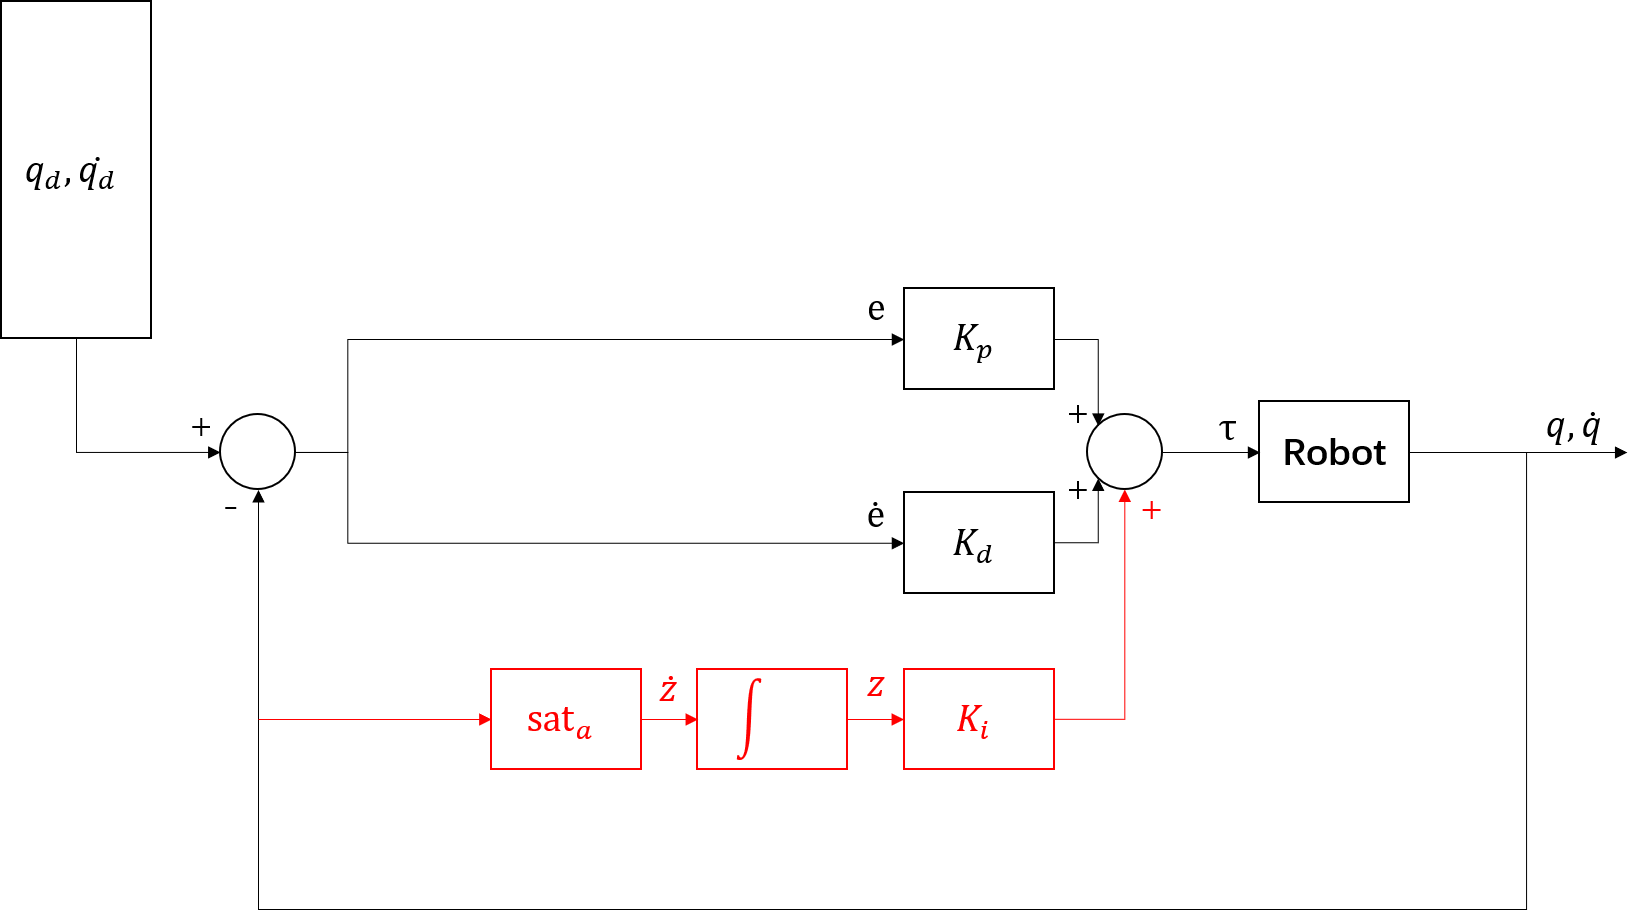
\includegraphics[width=0.7\linewidth]{pngs/Fig_6}
	\caption{PD control with integral-based compensation}
	\label{fig:fig6}
\end{figure}

\subsubsection{Integral-Based Method}

In the integral-based structure, gravity-related effects are compensated through an auxiliary dynamic state driven by the tracking error. The control law is given by
\begin{equation}
	\tau = -K_p e - K_d \dot{e} + K_i z,
\end{equation}
with the auxiliary state evolving as
\begin{equation}
	\dot{z} = \mathrm{sat}_{\alpha}(e),
\end{equation}
where $\mathrm{sat}_{\alpha}(\cdot)$ is a bounded nonlinear function. The purpose is to prevent integral saturation.

\section{Experimental Results}

The experiments are conducted on a six-degree-of-freedom mobile manipulator equipped with Mecanum wheels. All control algorithms are implemented on the real system, while performance metrics and sensitivity analyses are computed offline using the recorded experimental data. This setup allows direct observation of structural effects induced by different gravity compensation integration schemes under identical operating conditions.


\subsection{Experimental Setup}
All experiments are conducted on a six-degree-of-freedom mobile manipulator equipped with Mecanum wheels. Control laws are implemented on the real system, while performance indices are computed offline using recorded joint data.

The physical parameters of the manipulator are summarized in Table~\ref{tab:physical_params}, and the controller parameters and experimental settings are listed in Table~\ref{tab:control_exp_params}. Unless otherwise specified, identical PD gains and reference trajectories are used for all controllers to ensure that observed differences are primarily attributed to the gravity compensation integration structure.

To isolate gravity-dominated effects and avoid coupling-induced ambiguity, gain variations are applied only to the shoulder joint, where gravity torque is most significant. Gains of the remaining joints are fixed and their motions remain close to the reference throughout the experiments.


\begin{table}[t]
	\centering
	\caption{Physical Parameters of the Manipulator System}
	\label{tab:physical_params}
	\begin{tabular}{lll}
		\hline
		Parameter & Description & Value \\
		\hline
		$g$   & Gravitational acceleration & $9.81~\mathrm{m/s^2}$ \\
		$m_1$ & Mass of link 1              & $3.2~\mathrm{kg}$ \\
		$l_1$ & Length of link 1            & $0.36~\mathrm{m}$ \\
		$m_2$ & Mass of link 2              & $4.0~\mathrm{kg}$ \\
		$l_2$ & Length of link 2            & $0.27~\mathrm{m}$ \\
		$m_2$ & Mass of link 2              & $4.0~\mathrm{kg}$ \\
$l_2$ & Length of link 2            & $0.27~\mathrm{m}$ \\		
		$m_e$ & Payload mass     & $2.7~\mathrm{kg}$ \\
		$l_e$ & Wrist center-of-mass offset & $0.07~\mathrm{m}$ \\
		\hline
	\end{tabular}
\end{table}

\begin{table}[t]
	\centering
	\caption{Control Parameters and Experimental Settings}
	\label{tab:control_exp_params}
	\begin{tabular}{lll}
		\hline
		Parameter & Description & Value \\
		\hline
		$q_0$     & Target joint position        & $[0.6,\;0.3,\;1.4,\;0.7]~\mathrm{rad}$ \\
		$\dot q_0$& Initial joint velocity        & $\mathbf{0}$ \\
		$q_{\mathrm{ref}}$ & Reference joint position & $\mathbf{0}$ \\
		$f_{\mathrm{base}}$ & Base shaking frequency & $ 50\mathrm{Hz}$ \\
		$A_{\mathrm{base}}$ & Base shaking amplitude & $0.03\mathrm{m}$ \\
		$\Delta t$& Sampling period               & $0.1~\mathrm{s}$ \\
		$T$       & Experimental duration           & $50~\mathrm{s}$ \\
		$K_p$     & Proportional gain (joint 1)   & $10 \sim 75$ \\
		$K_d$     & Derivative gain (joint 1)     & $0.1 \sim 1.0$ \\
		$K_i$     & Integral gain (PD+NI)         & $\mathrm{diag}(1.3,0,0,0)$ \\
		$\alpha$  & NI filter parameter           & $0.8$ \\
		$G_{\max}$& Gravity saturation limit      & $[30,0,0,0]$ \\
		\hline
	\end{tabular}
\end{table}
Gain variations are applied only to the shoulder joint to isolate gravity-dominated dynamics, while gains of other joints are fixed.

\subsection{Evaluation Metrics}
 Different gravity-compensated integral structures implicitly emphasize different error paths, such as steady-state cancellation, transient decay, or dynamic disturbance suppression. Therefore, three representative performance metrics are used to reflect these structural characteristics.

Steady-state accuracy is given by the root-mean-square (RMS) tracking error over a steady-state window, denoted by $J_{\mathrm{ss}}$; transient behavior by the maximum moving average (MA) of the tracking error norm, $J_{\mathrm{ma}}$, capturing short-term amplification and oscillations; and convergence speed by fit to an exponential decay model.


The steady-state root-mean-square (RMS) tracking error is defined as
\begin{equation}
	J_{\mathrm{ss}} 
	= \sqrt{
		\frac{1}{|\mathcal{W}|}
		\sum_{k \in \mathcal{W}}
		\left\|
		q(k) - q_{\mathrm{ref}}
		\right\|^2
	},
\end{equation}
where $\mathcal{W}$ denotes the time window corresponding to the steady-state phase\cite{b13}.

The maximum moving-average tracking error is defined as
\begin{equation}
	J_{\mathrm{ma}}
	=
	\max_{t}
	\left(
	\frac{1}{\Delta T}
	\int_{t}^{t+\Delta T}
	\left\|
	q(\tau) - q_{\mathrm{ref}}
	\right\|
	\, d\tau
	\right),
\end{equation}
which characterizes the worst-case averaged tracking deviation over a sliding time window of length $\Delta T$ and reflects transient and oscillatory behaviors\cite{b14}.

To quantify the convergence speed, the tracking error norm is approximated by an exponential decay model
\begin{equation}
	\left\|
	e(t)
	\right\|
	\approx
	C e^{-\lambda t},
\end{equation}
where $\lambda$ represents the convergence rate and $C$ is a positive constant\cite{b15}.

\subsection{Results Analysis}

\begin{figure}
	\centering
	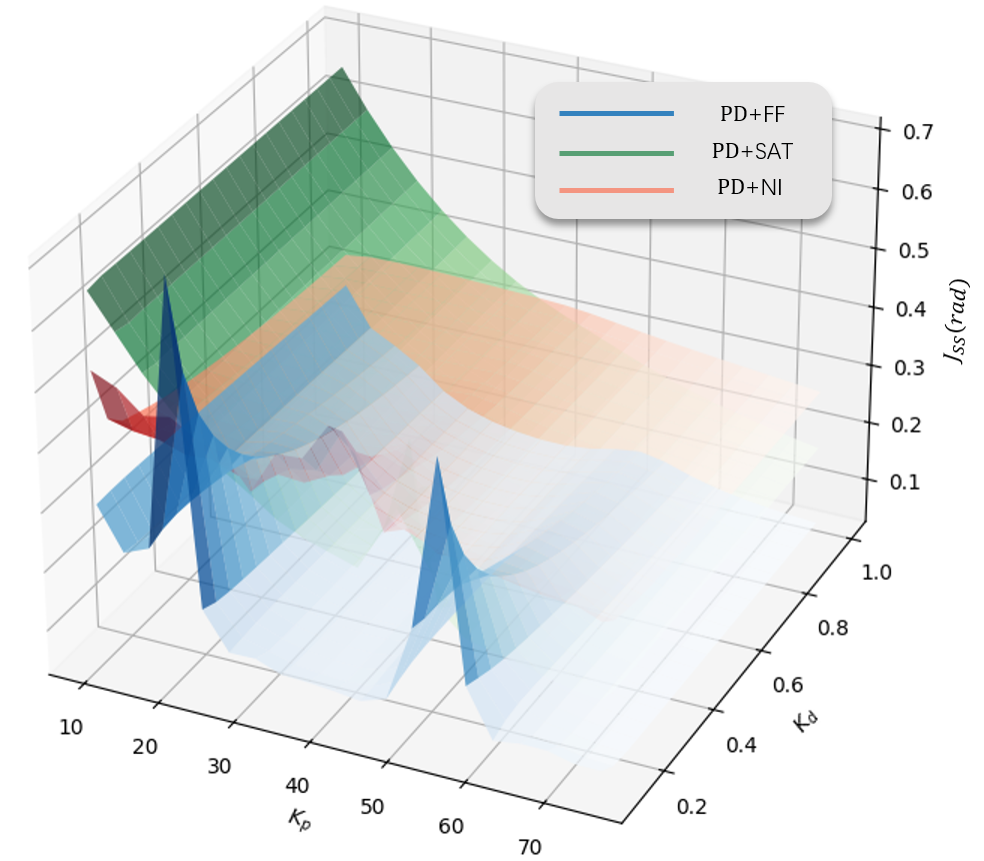
\includegraphics[width=0.8\linewidth]{pngs/figure1}
	\caption{Steady-state tracking errors under different compensation mechanisms.}
	\label{fig:fig7}
\end{figure}
Figure~\ref{fig:fig7} illustrates the steady-state tracking errors obtained under different gravity compensation integration structures. When the gravity model is accurate, additive feedforward compensation achieves lower steady-state RMS errors, reflecting its structural assumption that gravity can be treated as a known and cancelable deterministic term.

However, the residual error increases with parameter variations, indicating a direct correlation between steady-state performance and model accuracy. This phenomenon highlights the inherent sensitivity of treating gravity compensation as an explicit feedforward input rather than part of the feedback dynamics.

\begin{figure}
	\centering
	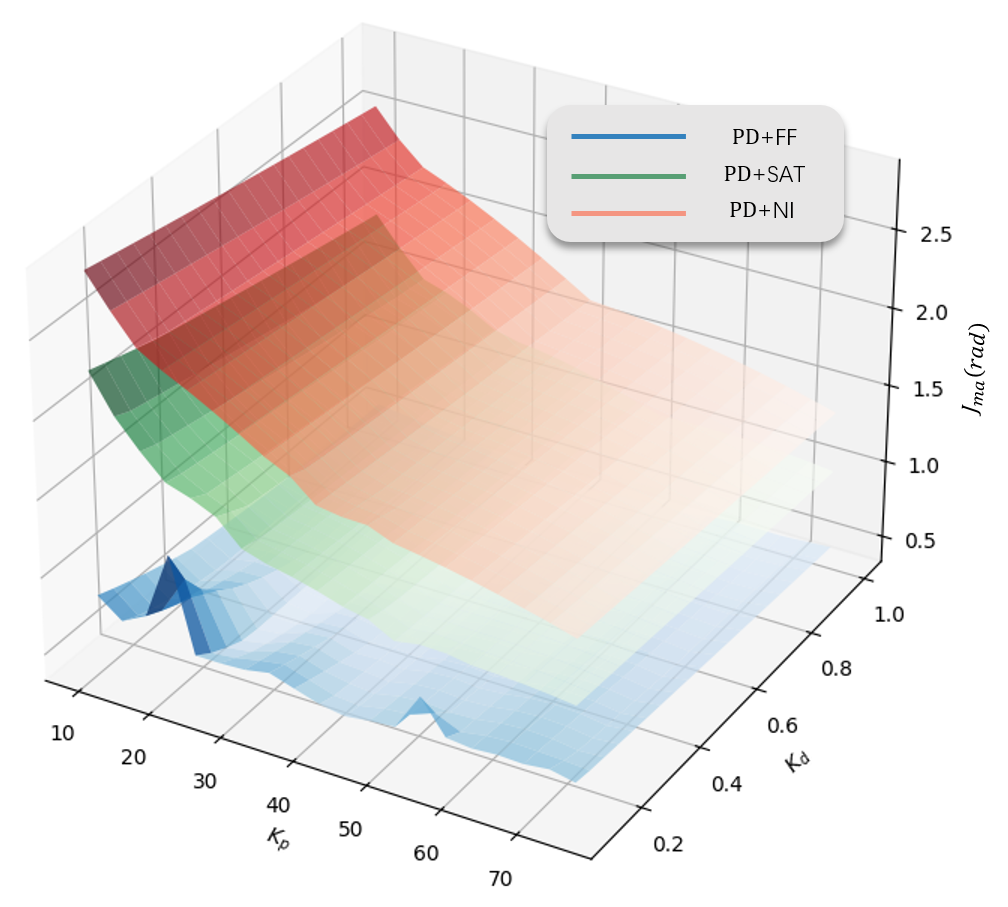
\includegraphics[width=0.8\linewidth]{pngs/figure2}
	\caption{Maximum moving-average tracking errors for different compensation mechanisms.}
	\label{fig:fig8}
\end{figure}


Figure~\ref{fig:fig8} shows the maximum moving average tracking error. Compared to the integral structure, saturation-based compensation limits the impact of gravity compensation on the control signal, thereby reducing transient error amplification.

The integral-based structure exhibits larger transient deviations, which can be attributed to the additional dynamics introduced by the integral state. Nevertheless, the absence of sustained oscillations suggests that steady-state regulation is structurally delegated to the integral action rather than enforced through precise gravity cancellation.

\begin{figure}
	\centering
	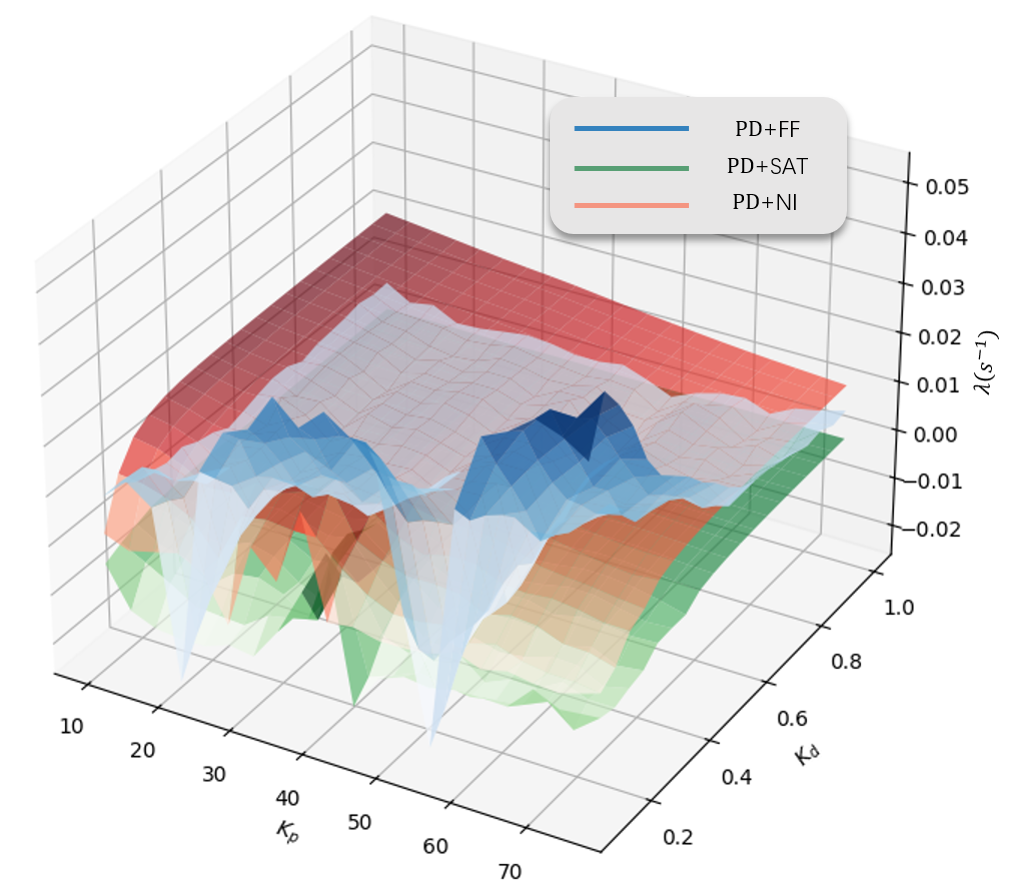
\includegraphics[width=0.8\linewidth]{pngs/figure3}
	\caption{Convergence rates of the tracking error under different compensation mechanisms.}
	\label{fig:fig9}
\end{figure}

The convergence rates estimated from the exponential error decay model are compared in Figure~\ref{fig:fig9}. When model parameters are well matched, additive feedforward compensation exhibits faster convergence, consistent with its direct gravity cancellation mechanism.

In contrast, saturation-based and integral-based structures exhibit slower but more consistent convergence behavior under different parameter settings. This reflects a structural trade-off: to reduce dependence on the accuracy of the gravity model, some convergence speed is sacrificed.

\begin{figure*}
	\centering
	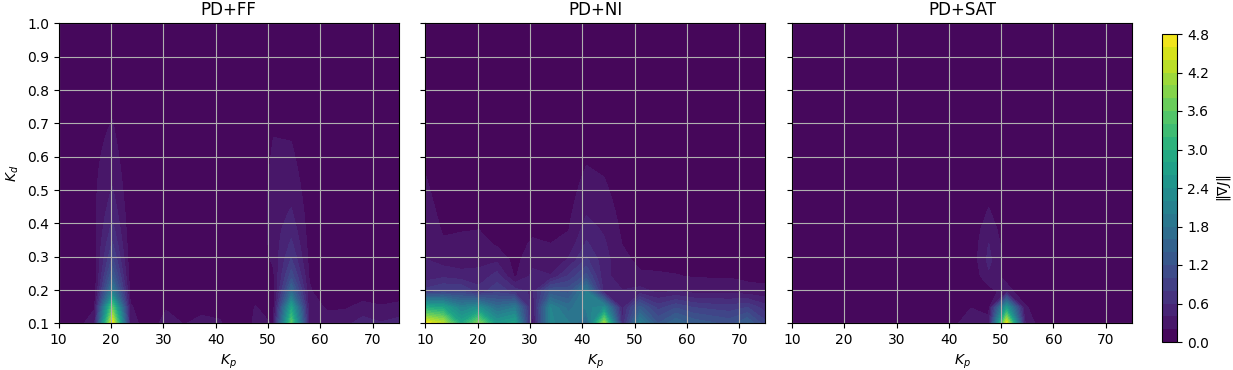
\includegraphics[width=1.0\linewidth]{pngs/Figure_4}
	\caption{Numerical gradient heat map of the steady-state error surface with respect to controller gains.}
	\label{fig:fig10}
\end{figure*}
Figure~\ref{fig:fig10} presents the numerical gradient heat map of the steady-state error surface with respect to controller gain variations. The additive feedforward structure exhibits steep gradients and narrow regions of low error, indicating that acceptable performance is confined to a limited tuning region.

In contrast, saturation-based and integral-based structures produce smoother error curves and have a wider acceptable performance range. This characteristic directly reflects their treatment of gravity as a bounded or implicitly compensable perturbation, rather than as a feedforward term for precise modeling.


Overall, the experimental results indicate that different gravity compensation integration structures lead to distinct and repeatable performance patterns in steady-state accuracy, transient response, convergence behavior, and gain sensitivity. These patterns are consistent with how gravity is structurally positioned within the control architecture, suggesting that gravity compensation should be regarded as a controller-level design choice rather than a purely implementation-level addition.

The results therefore support the central claim of this paper: gravity compensation should be regarded as a controller-level structural design choice, rather than as an auxiliary performance enhancement added to a given control law. These results indicate that performance metrics such as steady-state accuracy, convergence speed, and tuning robustness are not independent of controller structure, but are implicitly prioritized by how gravity compensation is positioned in the error dynamics.




\section{Lyapunov-Based Interpretation of Experimental Results}

\subsection{Unified Error Dynamics}
Consider the standard Euler--Lagrange model of an $n$-DOF robotic manipulator
\begin{equation}
	M(q)\ddot q + C(q,\dot q)\dot q + G(q) = \tau + d(t),
\end{equation}
where $d(t)$ denotes bounded disturbances induced by the mobile base.

Define the tracking error as $e = q - q_d$. For all gravity compensation integration structures considered in this paper, the closed-loop error dynamics can be written in the unified form
\begin{equation}
	M(q)\ddot e + C(q,\dot q)\dot e + K_d \dot e + K_p e
	= \Delta g(q) + d(t) + \Delta u,
	\label{eq:unified_error}
\end{equation}
where $\Delta g(q)=G(q)-\hat G(q)$ denotes gravity modeling error, and $\Delta u$ represents bounded nonlinear terms introduced by saturation or integral action.


\subsection{Lyapunov-Based Structural Interpretation}
Consider the Lyapunov candidate
\begin{equation}
	V = \frac{1}{2}\dot e^\top M(q)\dot e
	+ \frac{1}{2} e^\top K_p e .
\end{equation}

Using standard properties of Euler--Lagrange systems, the time derivative of $V$ along \eqref{eq:unified_error} satisfies
\begin{equation}
	\dot V \le - \lambda_{\min}(K_d)\|\dot e\|^2
	+ \|\dot e\|(\bar g + \bar d + \bar u),
\end{equation}
where $\bar g$, $\bar d$, and $\bar u$ denote bounds on gravity modeling error, external disturbances, and additional nonlinear terms, respectively.

From this inequality, the qualitative influence of different gravity compensation integration structures can be interpreted. For additive feedforward compensation, $\Delta u = 0$, and the ultimate bound is directly affected by gravity modeling error, explaining the fast convergence but high parameter sensitivity observed experimentally. For saturation-based compensation, $\Delta u$ is explicitly bounded by design, which limits the influence of gravity modeling inaccuracies and leads to smoother gain sensitivity at the cost of a nonzero steady-state error. For integral-based compensation, constant gravity-related disturbances are dynamically rejected through an additional internal state, ensuring zero steady-state error while introducing slower convergence due to additional dynamics.

\section{Conclusion}
This paper investigates gravity compensation within a PD control framework from the perspective of controller architecture. Through unified experimental comparisons, results show that different integrated gravity compensation structures lead to trade-offs in steady-state accuracy, transient response, convergence speed, and gain sensitivity. These results indicate that gravity compensation should be considered a controller-level structural design choice, rather than a simple implementation-level enhancement. In this sense, gravity compensation should be viewed as a controller architecture-level design choice that implicitly prioritizes performance, rather than a purely implementation-level enhancement added to a given control law. Future work will extend this framework to synchronous control for payload parameter estimation and gravity model adaptation. Furthermore, a Pareto-dominated structured multi-objective gain design framework will be investigated to formally explore the existence of an optimal controller gravity compensation design.




\begin{thebibliography}{00}

	\bibitem{b1}
	J.~H. Aylor, R.~L. Ramey, and G.~Cook,
	``Design and application of a microprocessor PID predictor controller,''
	\emph{IEEE Transactions on Industrial Electronics and Control Instrumentation},
	vol.~IECI-27, no.~3, pp.~133--137, Aug.~1980,
	doi: 10.1109/TIECI.1980.351665.
	
	\bibitem{b2}
	J.~J.~E. Slotine and W.~Li,
	\emph{Applied Nonlinear Control}.
	Englewood Cliffs, NJ, USA: Prentice-Hall, 1991.
	
	\bibitem{b3}
	C.~An, C.~Atkeson, and J.~Hollerbach,
	``Experimental determination of the effect of feedforward control on trajectory tracking errors,''
	in \emph{Proc. IEEE Int. Conf. on Robotics and Automation},
	San Francisco, CA, USA, 1986, pp.~55--60,
	doi: 10.1109/ROBOT.1986.1087669.
	
	\bibitem{b4}
	J.~J. Craig,
	\emph{Introduction to Robotics: Mechanics and Control},
	3rd~ed.
	Upper Saddle River, NJ, USA: Pearson Prentice Hall, 2005.
	
	\bibitem{b5}
	A.~Perrusqu\'{\i}a, J.~A. Flores-Campos, and C.~R. Torres-San-Miguel,
	``A novel tuning method of PD with gravity compensation controller for robot manipulators,''
	\emph{IEEE Access},
	vol.~8, pp.~114773--114783, 2020,
	doi: 10.1109/ACCESS.2020.3003842.
	
	\bibitem{b6}
	J.~Charaja, E.~Mu\~noz-Panduro, O.~E. Ramos, and R.~Canahuire,
	``Trajectory tracking control of UR5 robot: A PD with gravity compensation and sliding mode control comparison,''
	in \emph{Proc. Int. Conf. on Control, Automation and Diagnosis},
	Paris, France, 2020, pp.~1--5,
	doi: 10.1109/ICCAD49821.2020.9260559.
	
	\bibitem{b7}
	C.~An, C.~Atkeson, J.~Griffiths, and J.~Hollerbach,
	``Experimental evaluation of feedforward and computed torque control,''
	in \emph{Proc. IEEE Int. Conf. on Robotics and Automation},
	Raleigh, NC, USA, 1987, pp.~165--168,
	doi: 10.1109/ROBOT.1987.1088020.
	
	\bibitem{b8}
	A.~Zavala-R\'{\i}o and V.~Santib\'a\~nez,
	``A natural saturating extension of the PD-with-desired-gravity-compensation control law for robot manipulators with bounded inputs,''
	\emph{IEEE Transactions on Robotics},
	vol.~23, no.~2, pp.~386--391, Apr.~2007,
	doi: 10.1109/TRO.2007.892224.
	
	\bibitem{b9}
	R.~Kelly,
	``Global positioning of robot manipulators via PD control plus a class of nonlinear integral actions,''
	\emph{IEEE Transactions on Automatic Control},
	vol.~43, no.~7, pp.~934--938, Jul.~1998,
	doi: 10.1109/9.701091.
	
	\bibitem{b10}
	F.~Liu and E.~M. Joo,
	``Linear and nonlinear PD-type control of robotic manipulators for trajectory tracking,''
	in \emph{Proc. IEEE Conf. on Industrial Electronics and Applications},
	Xi'an, China, 2009, pp.~3442--3447,
	doi: 10.1109/ICIEA.2009.5138846.
	
	\bibitem{b11}
	D.~Zhao, S.~Li, and F.~Gao,
	``Improvements on saturating PD with gravity compensation control for robotic manipulators,''
	in \emph{Proc. 7th Asian Control Conf.},
	Hong Kong, China, 2009, pp.~1497--1502.
	
	\bibitem{b12}
	V.~Santib\'a\~nez and R.~Kelly,
	``A class of nonlinear PID global regulators for robot manipulators,''
	in \emph{Proc. IEEE Int. Conf. on Robotics and Automation},
	Leuven, Belgium, 1998, pp.~3601--3606,
	doi: 10.1109/ROBOT.1998.681026.
	
	\bibitem{b13}
	Z.~Lv, D.~Ning, P.~Liu, and P.~Liao,
	``PD control with gravity compensation for 3-RPS parallel manipulator,''
	in \emph{Proc. IEEE Data Driven Control and Learning Systems Conf.},
	Xiangtan, China, 2023, pp.~1744--1749,
	doi: 10.1109/DDCLS58216.2023.10167077.
	
	\bibitem{b14}
	J.~J. Craig, J.~Hsu, and S.~S. Sastry,
	``Adaptive control of mechanical manipulators,''
	\emph{IEEE Transactions on Automatic Control},
	vol.~32, no.~1, pp.~54--59, Jan.~1987,
	doi: 10.1109/TAC.1987.1104506.
	
	\bibitem{b15}
	B.~Paden and R.~Panja,
	``Globally asymptotically stable ``PD+'' controller for robot manipulators,''
	\emph{International Journal of Control},
	vol.~47, no.~6, pp.~1697--1712, 1988,
	doi: 10.1080/00207178808906130.
	
	\bibitem{b16}
	M.~W. Spong, S.~Hutchinson, and M.~Vidyasagar,
	\emph{Robot Modeling and Control}.
	New York, NY, USA: Wiley, 2006.
	
\end{thebibliography}


\end{document}
